\documentclass[italian]{beamer}

%%% Dichiarazione dei pacchetti standard.
\usepackage{units}
\usepackage{babel}
\usepackage[utf8x]{inputenc}
\usepackage{subfigure}
\usepackage{graphicx}    % inclusione graph images )
\usepackage{url}
\usepackage{lmodern}
\usepackage{booktabs}
\usepackage[T1]{fontenc}
\usepackage{import}
\usepackage{xspace}
\usepackage{macros}
%gets rid of bottom navigation bars

\usetheme{Boadilla}
\usecolortheme{wolverine}

\setbeamertemplate{footline}[frame number]{}
\setbeamertemplate{navigation symbols}{} 
\graphicspath{{../../images/pdf/}}
    
%%% Titolo e autore.
\title[Ricerca di partner del top]{Ricerca di particelle esotiche di carica
    \nicefrac{5}{3} a CMS}
\author{Matteo Abis\\
\url{matteo.abis@cern.ch}}
\institute{Università di Padova}
\date{\today}

\begin{document}

\begingroup
\begin{frame}
  \titlepage
\end{frame}
\endgroup
 
\begin{frame}
    \frametitle{Il problema della gerarchia nel modello standard}
    \begin{figure}[h]
        \centering
        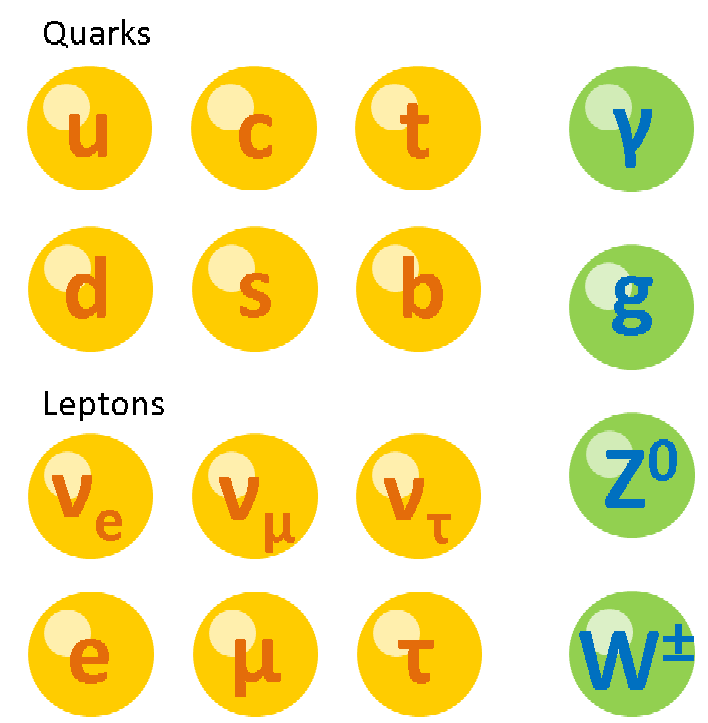
\includegraphics[width=.5\textwidth]{standard_model_particles}
    \end{figure}
\end{frame}
\begin{frame}
    \frametitle{Il problema della gerarchia nel modello standard}
    \begin{block}
        {Problema di naturalezza}
        La massa del bosone di Higgs riceve grandi contributi da diagrammi
        con un \emph{loop}. Per avere una massa piccola \`e
        necessaria una incredibile calibrazione fine dei parametri del
        modello standard. 
    \end{block}
    \begin{figure}[h]
        \centering
        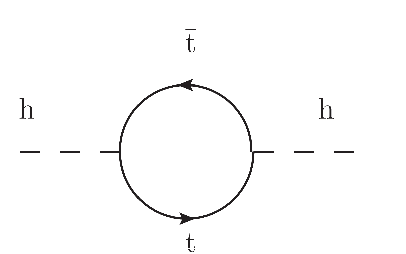
\includegraphics[height=.4\textheight]{higgs_correction}
    \end{figure}
\end{frame}

\begin{frame}
    \frametitle{Partner del quark top}
    \framesubtitle{Una possibile estensione del modello standard}
    \begin{itemize}
        \item soluzione al problema della gerarchia
            \begin{itemize}
                \item \emph{Contino, Servant}, JHEP 0806:026 (2008)
                \item \emph{Mrazek, Wulzer}, Phys. Rev. D81, 075006 (2010)
            \end{itemize}
        \item produzione di coppie di $\mathrm{T}_{5/3}$
        \item decadimento in quark top e bosone $\mathrm{W}$
        \item \alert{firma sperimentale: due elettroni o muoni di alta energia e
                stessa carica, insieme a molti \emph{jet}.}
    \end{itemize}
    \begin{figure}[h]
        \centering
        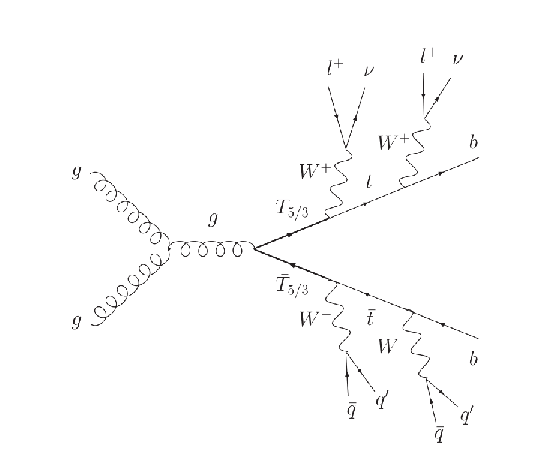
\includegraphics[height=.5\textheight]{TTbar_feynman}
    \end{figure}
\end{frame}
\begin{frame}
    \frametitle{Partner del quark top}
    \begin{figure}[h]
        \centering
        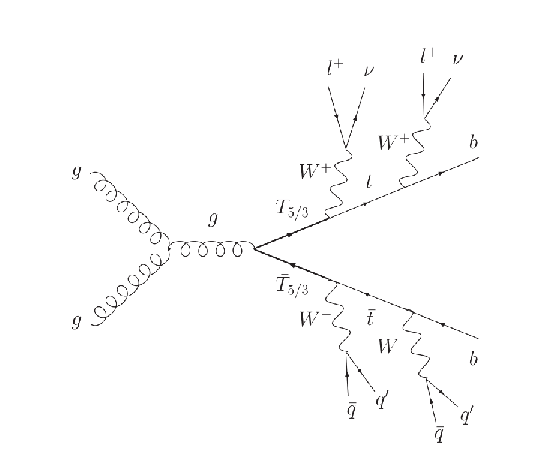
\includegraphics[height=.8\textheight]{TTbar_feynman}
    \end{figure}
\end{frame}

\begin{frame}
    \frametitle{Il rivelatore CMS}
    dati di CMS del
            2011 a $\sqrt{s} = \unit[7]{TeV}$\\
            luminosit\`a integrata
            $\unit[5]{fb^{-1}}$                          
            \begin{figure}[h]
                \centering
                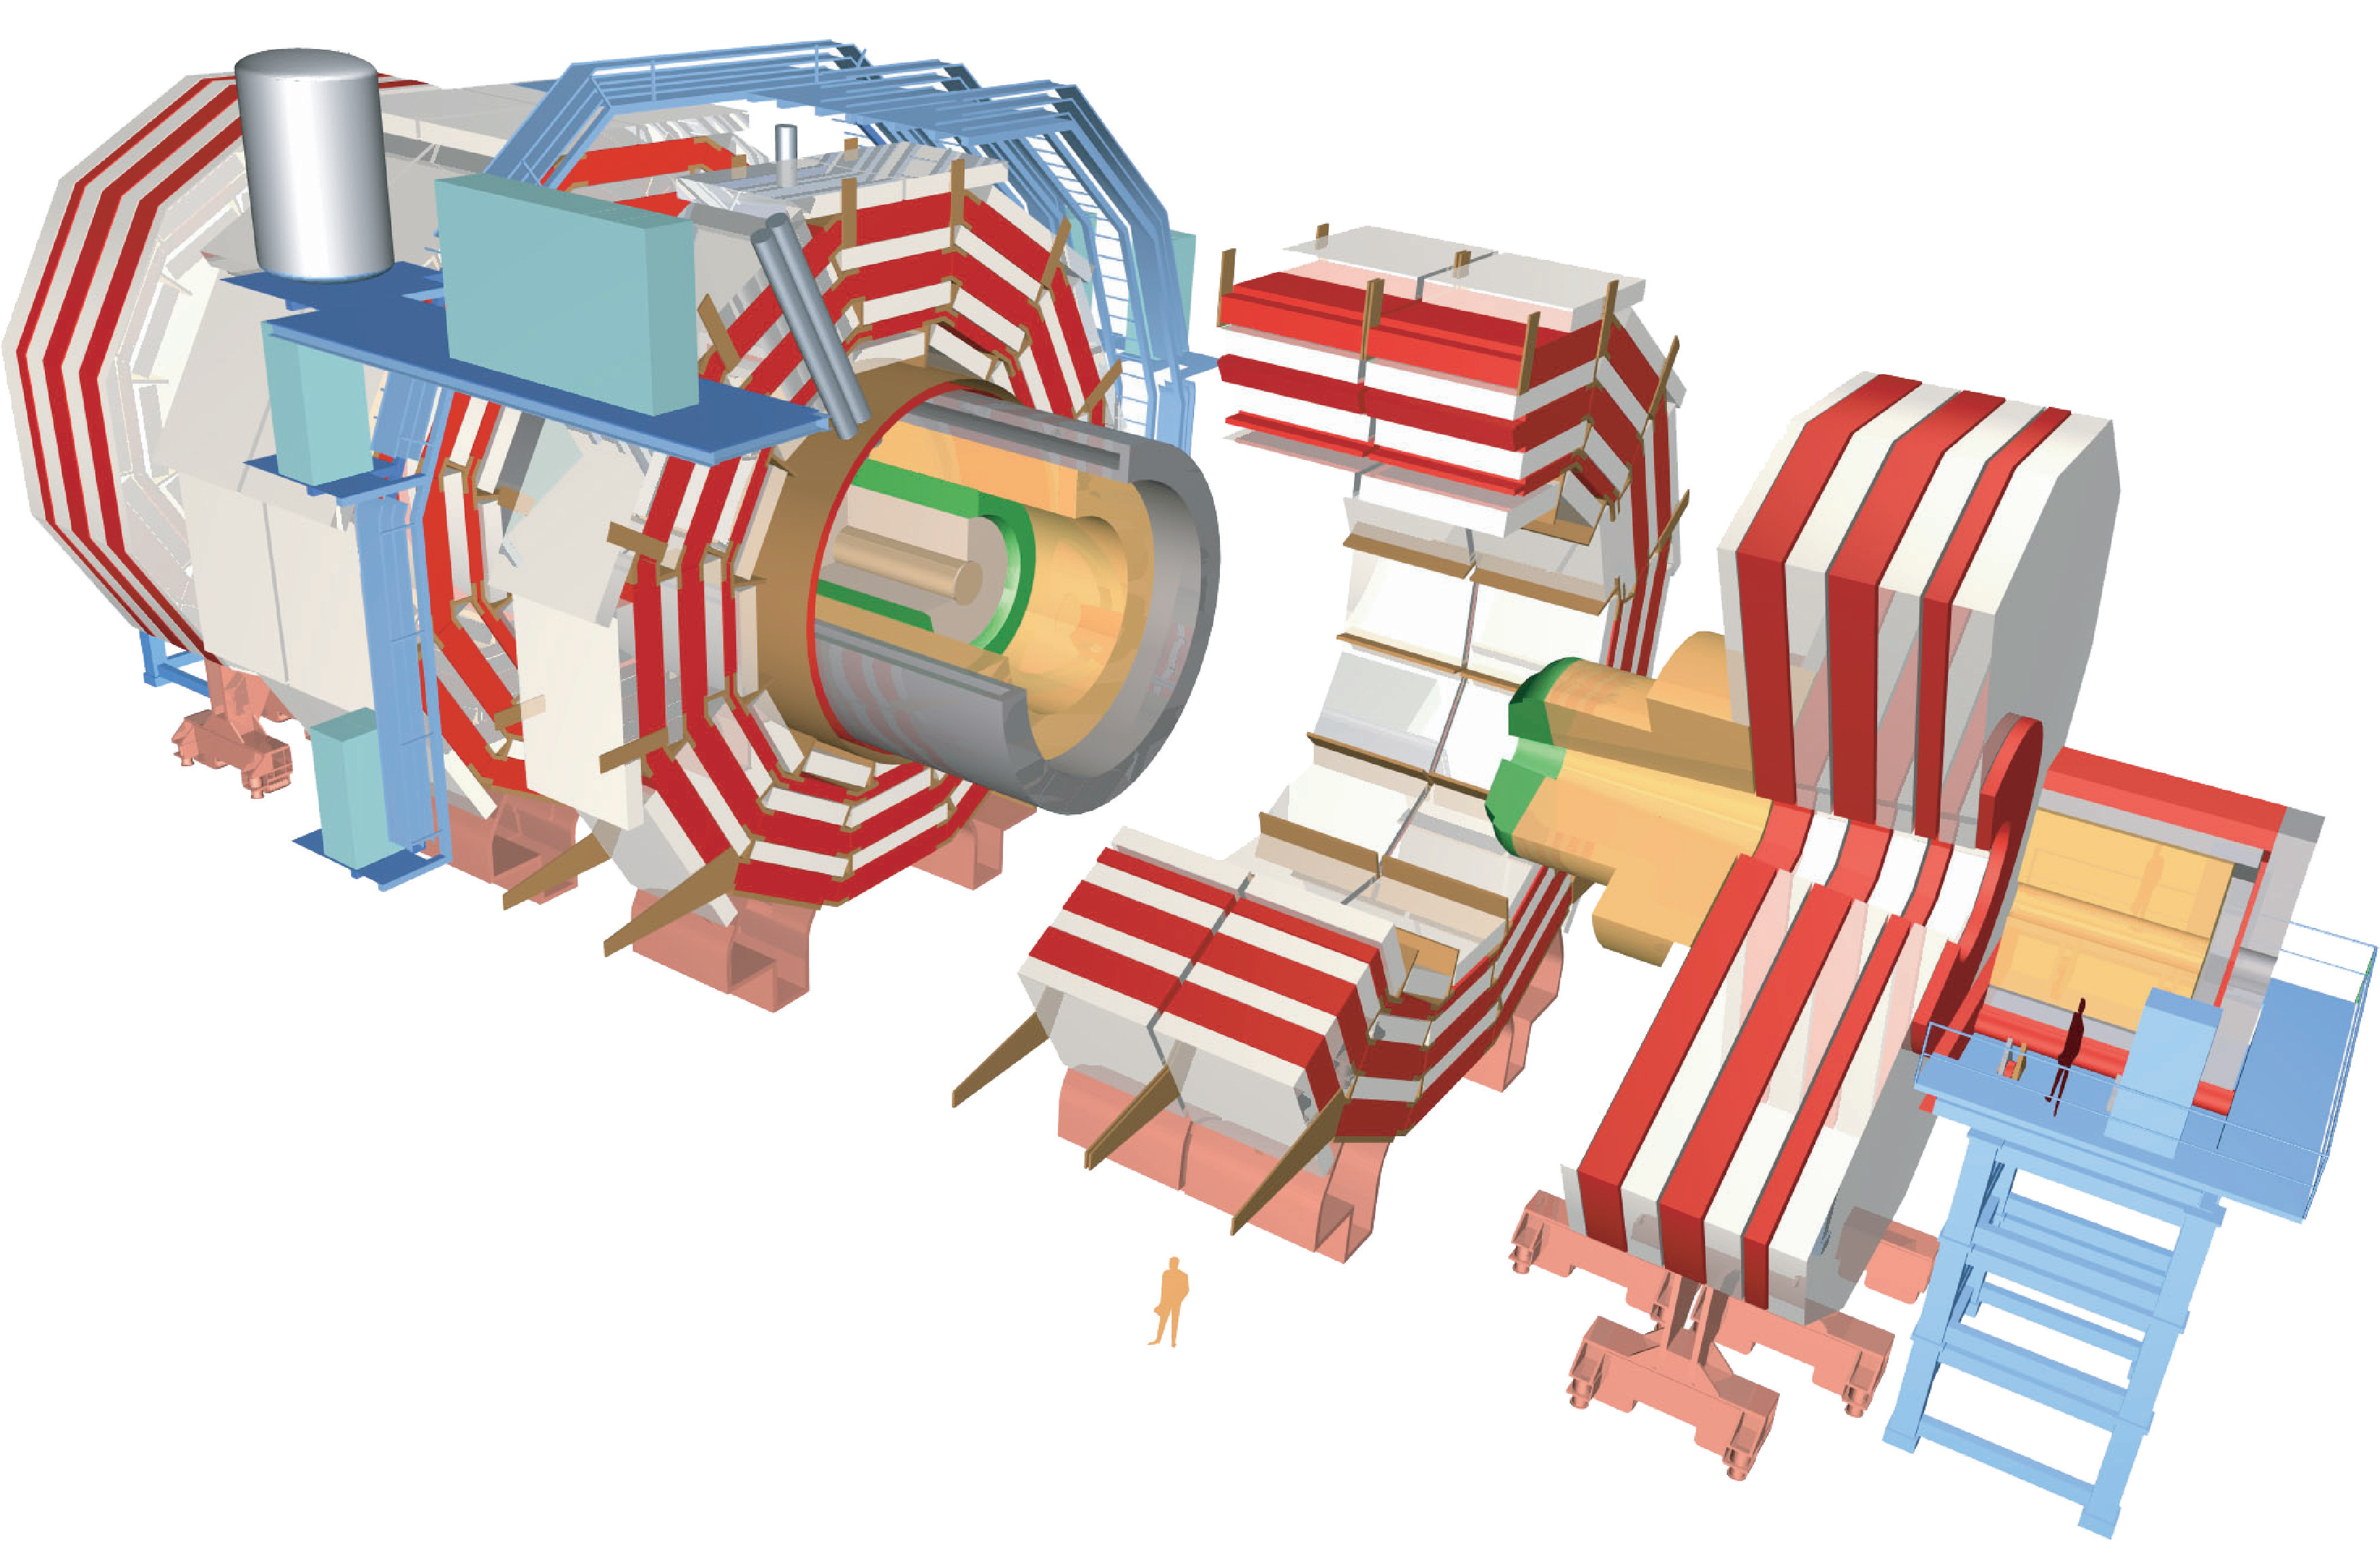
\includegraphics[width=.7\textwidth]{Schematic}
            \end{figure}
\end{frame}

\begin{frame}
    \frametitle{Fondi strumentali e di modello standard}
    Sezione d'urto del segnale: 
    \begin{table}
        \centering
        \begin{tabular}{cc}
            massa (GeV) & $\sigma \times \text{BR (fb)}$\\
            500 & 69 \\
            600 & 19 \\
            700 & 6 \\
        \end{tabular}
    \end{table}
    Due leptoni isolati, di alta energia e dello stesso segno possono essere dati da:
    \begin{enumerate}
        \item processi rari del modello standard con lo stesso stato finale.
        \item errata misura della carica di stati finali con leptoni di
            segno opposto.
        \item processi con decadimenti secondari, soprattutto il decadimento
            semileptonico del quark $\mathrm{b}$ dalla produzione di
            $\mathrm{t} \bar{\mathrm{t}}$.  
    \end{enumerate}
\end{frame}

\begin{frame}
    \frametitle{Processi rari del modello standard}
    Produzione di top insieme a un bosone vettore, o di pi\`u bosoni vettori
    contemporaneamente:
    $\mathrm{t} \bar{\mathrm{t}}\mathrm{Z}$, $\mathrm{t}
    \bar{\mathrm{t}} \mathrm{W}$,
                    $\mathrm{WW}$, $\mathrm{WZ}$, $\mathrm{ZZ}$ e
                    $\mathrm{WWW}$.

                    \alert{Simulati con tecniche Monte Carlo}
\end{frame}

\begin{frame}
    \frametitle{Errata misura della carica elettrica}
    \framesubtitle{Contributo stimato dai dati}
    \begin{description}
        \item[Selezione di candidati $\mathrm{Z}$:]
      coppie
    di leptoni con massa invariante tra \unit[76]{GeV} e
    \unit[106]{GeV}.
\item[Campione dominato al 99\% da $\mathrm{Z}$:] 
    le coppie con leptoni dello stesso segno vengono da una misura errata.
    \end{description}
    \begin{figure}[h]
        \centering
        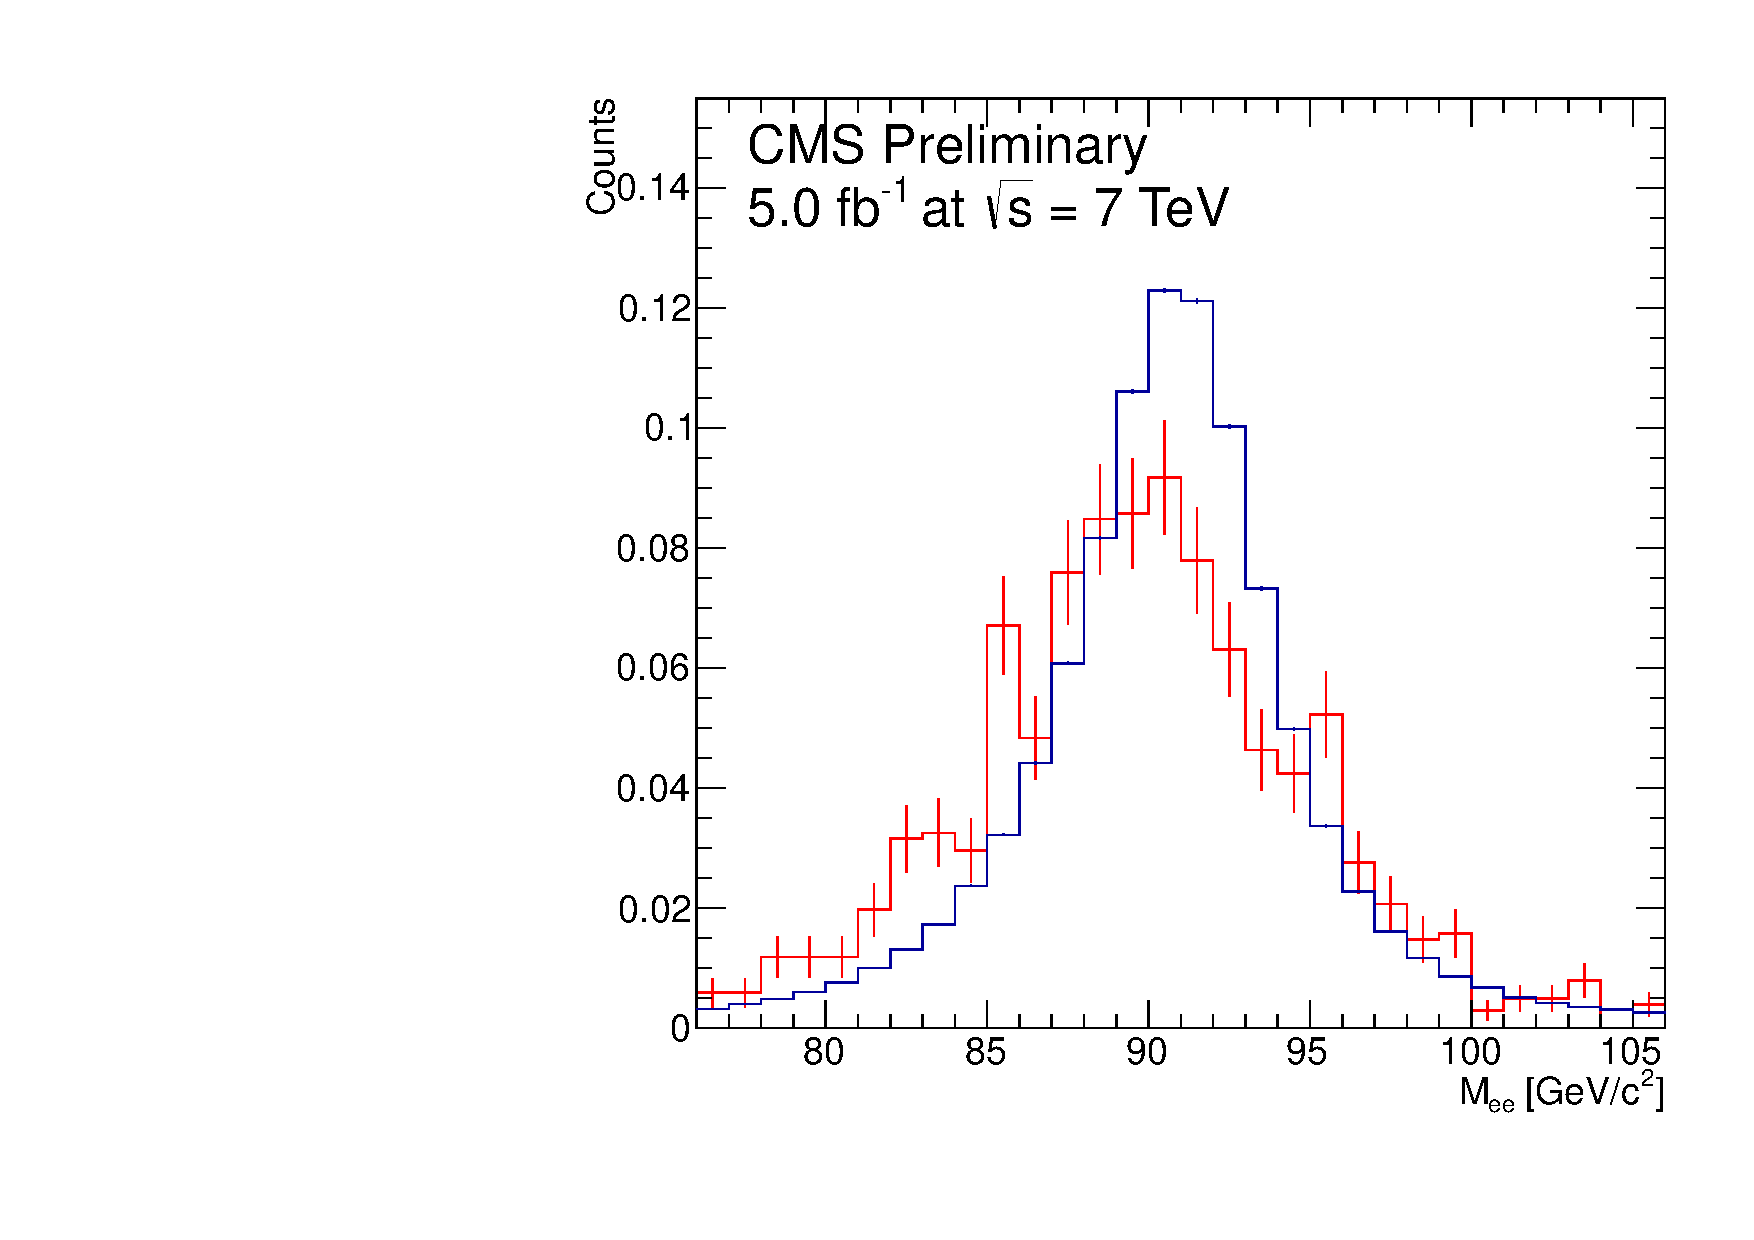
\includegraphics[height=.5\textheight]{ChargeMisID_ZMass}
        \caption{Distribuzione della massa invariante degli elettroni di segno
        opposto (blu) o dello stesso segno (rosso)}
    \end{figure}
\end{frame}

\begin{frame}
    \frametitle{Leptoni dello stesso segno da decadimenti secondari}
    \framesubtitle{Stima dai dati con il metodo \emph{tight-loose}}
    \begin{itemize}
        \item si definisce una categoria di leptoni con selezioni pi\`u
            lasche
        \item si misura la probabilit\`a che un leptone che passa questa
            selezione passi erroneamente anche quella, pi\`u stringente, dell'analisi
        \item dalla probabilit\`a si stima il numero di eventi
            che contaminano il campione finale
    \end{itemize}
    \begin{figure}[h]
        \centering
        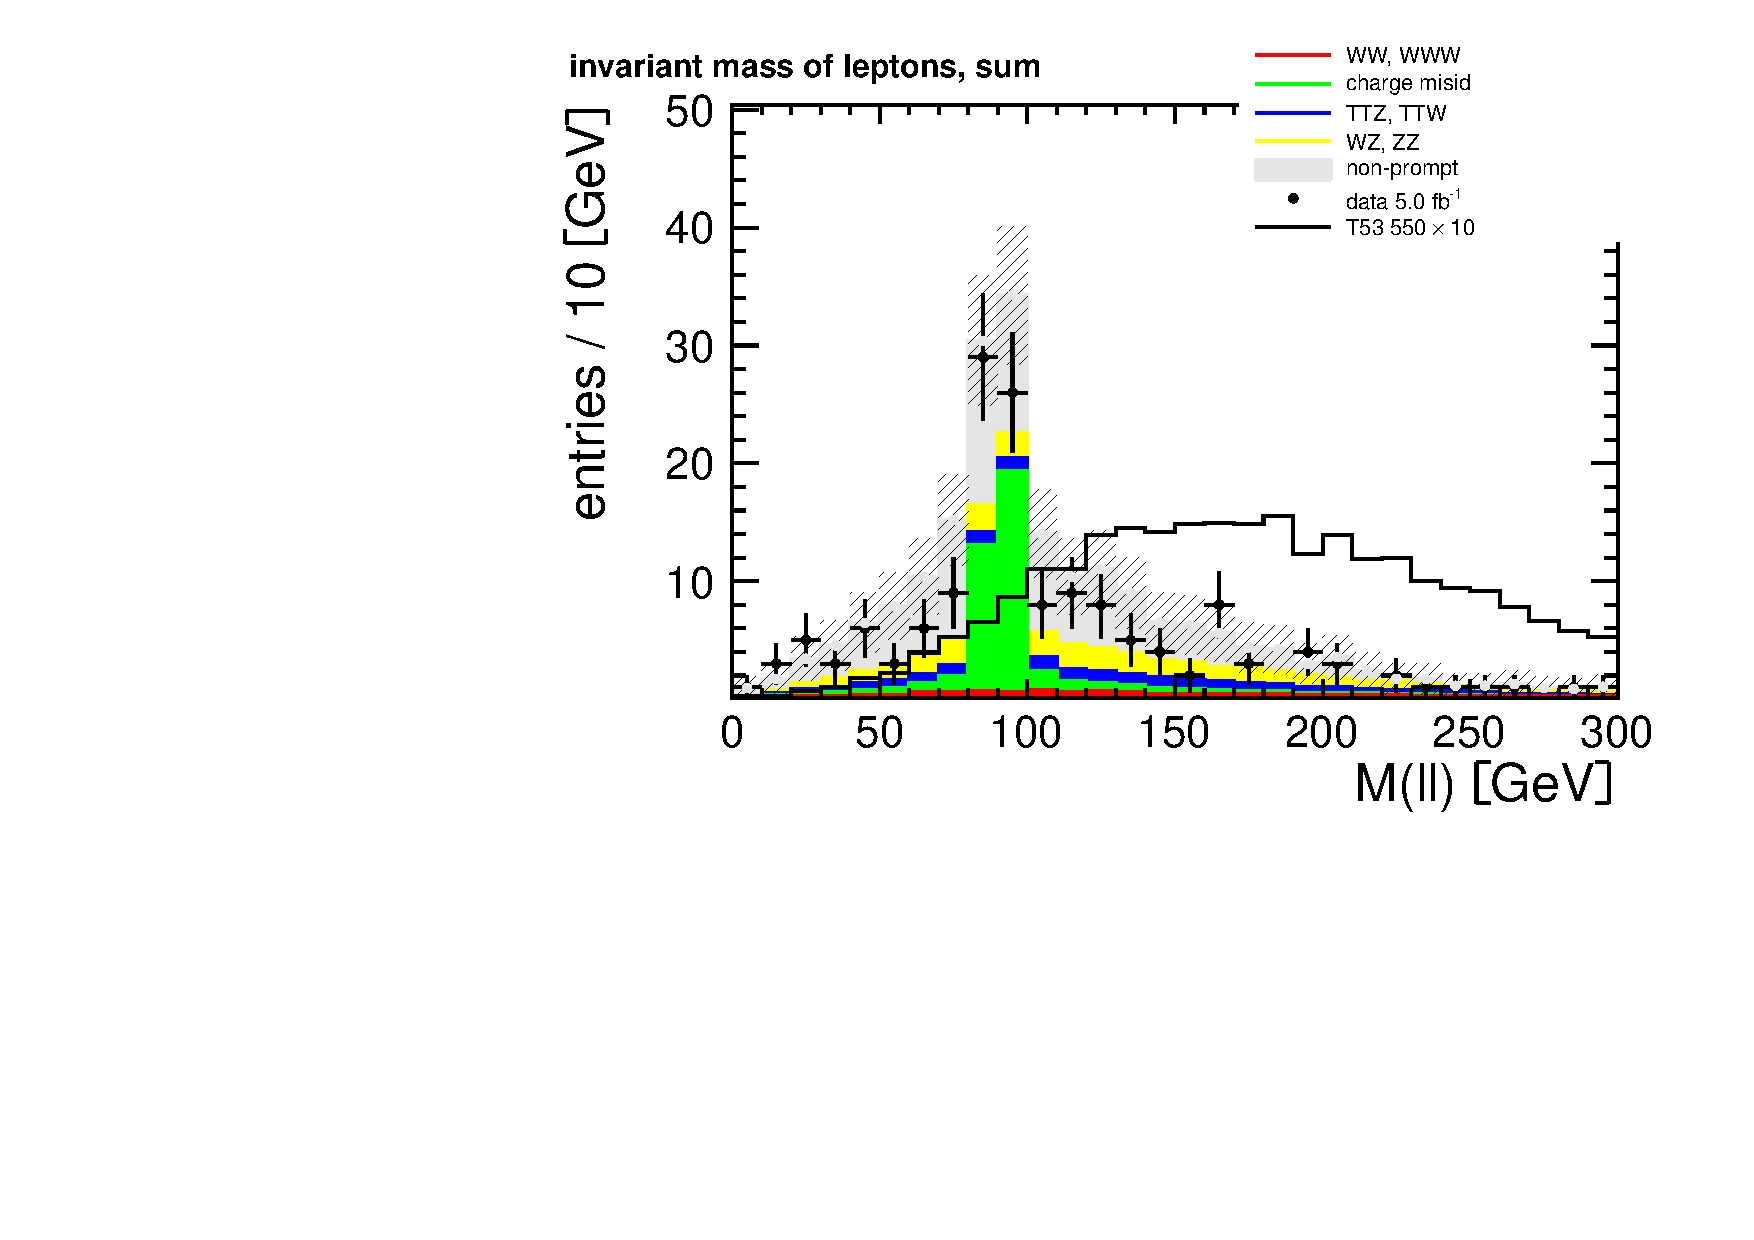
\includegraphics[width=.5\textwidth]{lep_mass_sum_1}
        \caption{Distribuzione della massa invariante dei due leptoni dello
        stesso segno in eventi con almeno due jet.}
    \end{figure}
\end{frame}

\begin{frame}
    \frametitle{Le variabili \emph{razor}}
    \begin{block}{Versione originale}
        Due particelle pesanti prodotte in coppia decadono in una particella
        visibile e una invisibile.\end{block}
    \begin{block}
        {Prima approssimazione}
        \begin{align*}
            M_R &= \sqrt{(a^0 + b^0)^2 - (a^z + b^z)^2} \\
            M_R^T &= \sqrt{\dfrac{|\vec{m}|}{2} (|\vec{a}_T| + |\vec{b}_T|) 
            -\dfrac{\vec{m}}{2} \cdot (\vec{a} + \vec{b})}\\
            R &= M_R^T / M_R
        \end{align*}
    \end{block}
    Notazione:
    \begin{itemize}
        \item $a^\mu$ e $b^\mu$ quadrivettori delle particelle visibili
        \item $\vec{m}$ \`e l'energia mancante nel piano trasverso \met
        \item $\vec{v}_T$ \`e un vettore con le componenti trasverse $(v_x, v_y, 0)$
    \end{itemize}
\end{frame}

\begin{frame}
    \frametitle{Propriet\`a delle variabili \emph{razor}}
    \begin{description}
        \item[$M_R$] indipendente da \emph{boost} lungo l'asse $z$,
            correlata con la massa dell'oggetto originale
        \item[$R$] altra misura indipendente della scala di energia del
            processo, che utilizza le misure sul piano trasverso
    \end{description}

    \begin{block}
        {Correzioni aggiuntive}
        Le formule sono corrette per il \emph{boost} complessivo del sistema applicando
        una trasformazione di Lorentz che porta nel sistema a riposo di $\vec{a} + \vec{b} +
        \vec{m}.$
    \end{block}
\end{frame}

\begin{frame}
    \frametitle{Il sottosistema \emph{razor}}
    \alert{La topologia del decadimento del partner del top \`e asimmetrica}

    \uncover<2->{
        \begin{figure}[h]
            \centering
            \subfigure[Esempio standard dalla supersimmetria]{
                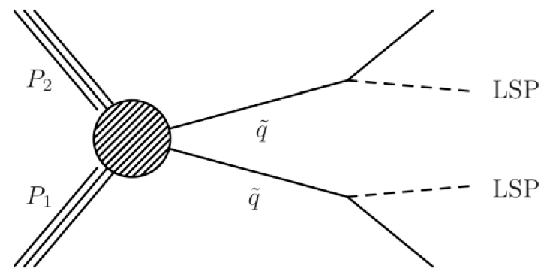
\includegraphics[width=.4\textwidth]{standard_razor_susy}}
                \subfigure[Evento con partner del
                top]{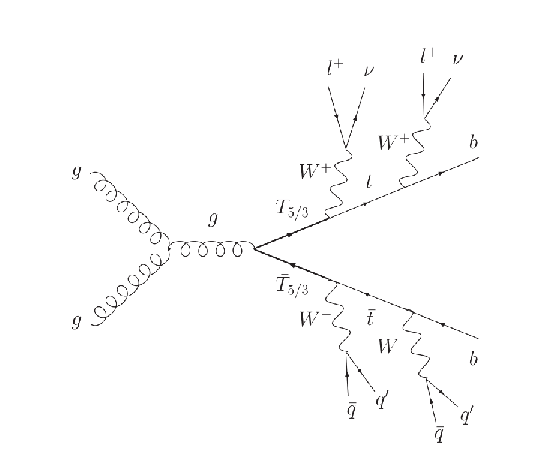
\includegraphics[width=.4\textwidth]{TTbar_feynman}}
        \end{figure}
    }
\end{frame}

\begin{frame}
    \frametitle{Massa invariante adronica}
    \framesubtitle{La parte pi\`u semplice}
    \begin{block}{}
        Massa della somma dei quadrimomenti dei jet
    \end{block}
        \begin{figure}[h]
            \centering
            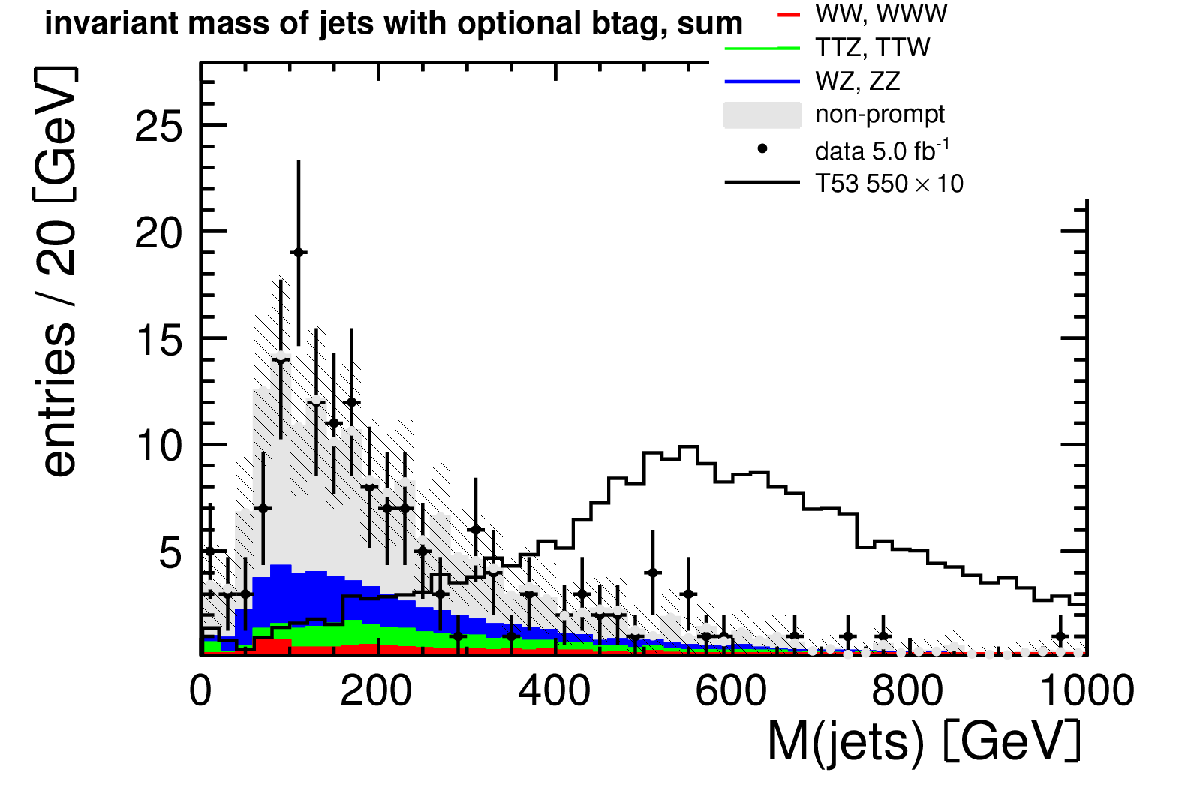
\includegraphics[width=.7\textwidth]{had_mass_optional_btag_sum}
        \end{figure}
\end{frame}

\begin{frame}
    \frametitle{$M_R$}
    \framesubtitle{Indicatore della massa della particella massiva}
    \begin{block}{}
        Picco previsto intorno a $M(\mathrm{T}_{5/3})/2$.
    \end{block}
        \begin{figure}[h]
            \centering
            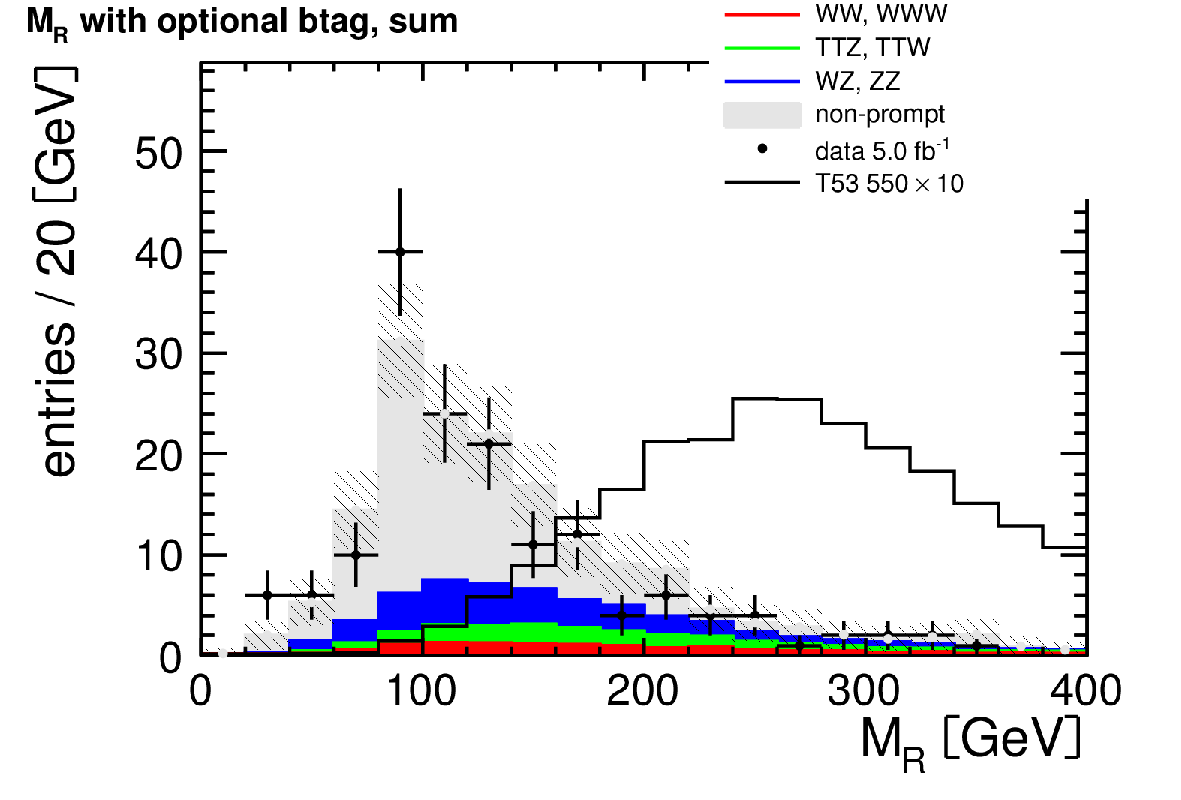
\includegraphics[width=.7\textwidth]{mr_optional_btag_sum}
        \end{figure}
\end{frame}

\begin{frame}
    \frametitle{$R$}
    \framesubtitle{Una variabile dimensionale correlata con la \met}
    In teoria:
    \begin{itemize}
        \item picco vicino a \nicefrac{1}{2} per il segnale
        \item decade esponenzialmente per i fondi dopo aver raggiunto un
            massimo
    \end{itemize}
        \begin{figure}[h]
            \centering
            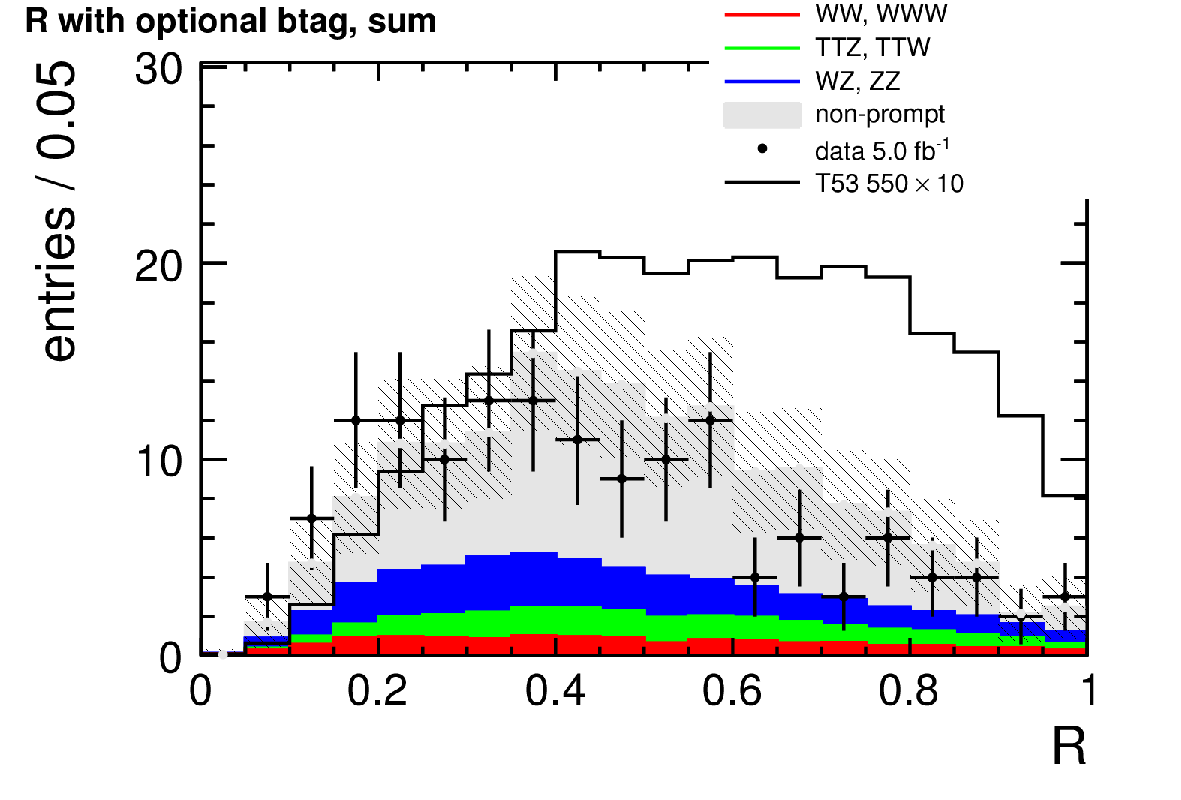
\includegraphics[width=.7\textwidth]{r_optional_btag_sum}
        \end{figure}
\end{frame}

\begin{frame}
    \frametitle{Un miglior rapporto segnale-rumore}
    Selezione finale ottimizzata per $S/(a + \sqrt{B})$. 
    \begin{itemize}
        \item massa adronica $>\unit[350]{GeV}$
        \item $M_R > \unit[200]{GeV}$
        \item $R > 0.2$
    \end{itemize}
\end{frame}

\begin{frame}
    \frametitle{Limite}
    Non si osserva un eccesso di eventi rispetto ai fondi del
    modello standard:
    \subimport{../../tables/}{expected}
    \alert{limite osservato (atteso)} \unit[633 (658)]{GeV}
    \begin{figure}[h]
        \centering
    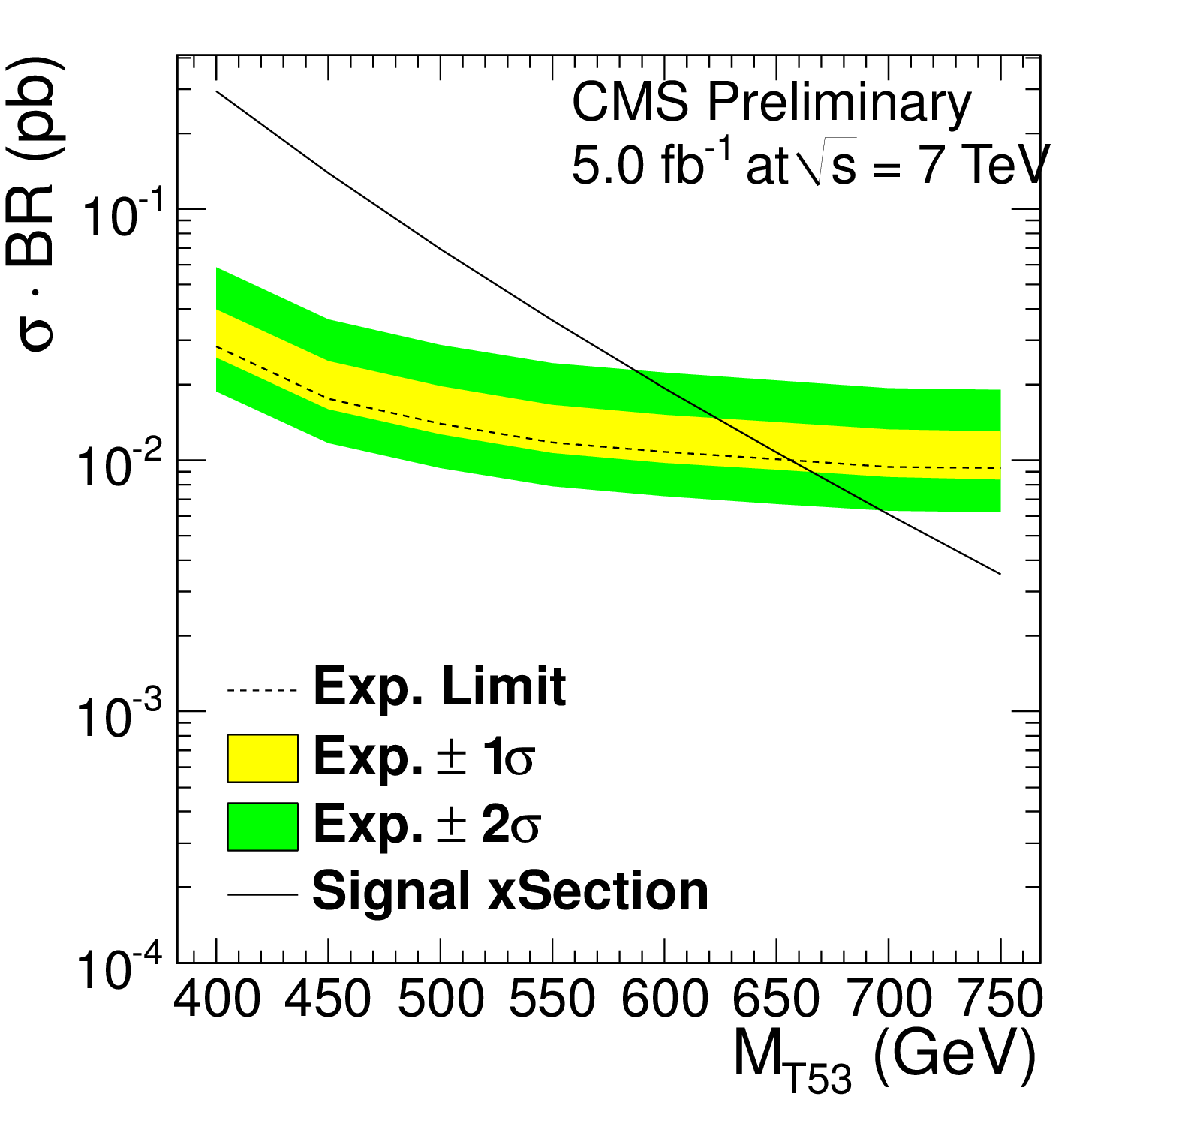
\includegraphics[height=.55\textheight]{oLimit_limit_macro_4jets_opt_btag_200_350_02}
        \caption{Limite al 95\% CL.}
    \end{figure}
\end{frame}

\begin{frame}
    \frametitle{Backup slides}
\end{frame}

\begin{frame}
    \frametitle{Signal MC}
    \framesubtitle{Fall11 production}
    \subimport{../../tables/}{signal_mc}
\end{frame}

\begin{frame}
    \frametitle{Background MC}
    \framesubtitle{Summer11 production}
    \subimport{../../tables/}{background_mc}
\end{frame}

\begin{frame}
    \frametitle{Data}
    \framesubtitle{2011 golden JSON, \unit[5.0]{$fb^{-1}$}}
    \subimport{../../tables/}{data_pd}
\end{frame}

\begin{frame}
    \frametitle{Triggers}
    \subimport{../../tables/}{triggers}
\end{frame}

\begin{frame}
    \frametitle{Event cleanup}
    \framesubtitle{Standard from TLBSM recipes}
    \begin{description}
        \item[scraping]\hspace*{\fill}\\
            \begin{itemize}
                \item at least 25\% of the tracks must be high-purity for events
            with at least ten tracks
            \end{itemize}
        \item[good primary vertex] \hspace*{\fill}\\
            \begin{itemize}
                \item at least 4 degrees of freedom
                \item less than \unit[25]{cm} from interaction point in $z$
                \item less than \unit[2]{cm} radially
            \end{itemize}
        \item[HBHE noise filter] 
    \end{description}
\end{frame}

\begin{frame}
    \frametitle{Electrons}
    \framesubtitle{Standard top selection, plus charge consistency}
    \begin{itemize}
        \item $\pt > \unit[30]{GeV}$
        \item $|\eta| < 2.4$, except EBEE gap
        \item HyperTight1MC electron identification
        \item relative isolation $< 0.15$
        \item conversion rejection
        \item transverse impact parameter $< \unit[0.02]{cm}$
        \item GSF, CFT, ScPix charge consistency
    \end{itemize}
\end{frame}

\begin{frame}
    \frametitle{Muons}
    \framesubtitle{Standard top selection}
    \begin{itemize}
        \item $\pt > \unit[30]{GeV}$
        \item $|\eta| < 2.4$
        \item Global and Tracker muon
        \item relative isolation $< 0.20$
        \item $\chi^2/\text{NDF} < 10$
        \item at least one muon hit
        \item at least one pixel hit
        \item at least eleven silicon hits
        \item at least two chambers with matching segments
    \end{itemize}
\end{frame}

\begin{frame}
    \frametitle{Jets}
    \framesubtitle{Standard top selection}
    \begin{itemize}
        \item anti-$k_T$ particle flow jets
        \item $\pt > \unit[30]{GeV}$
        \item $|\eta| < 2.4$
        \item Charged hadron subtractions, L1FastJets corrections,
            L2L3 jet energy scale corrections
        \item loose particle flow identification
        \item $\Delta R(\text{lepton, jet}) > 0.3$
    \end{itemize}
\end{frame}
\end{document}
